\documentclass[tikz,border=8pt]{standalone}
% Shared look for every TikZ diagram. Load with % Shared look for every TikZ diagram. Load with % Shared look for every TikZ diagram. Load with \input{../../tools/tikz-style.tex}
\usepackage[T1]{fontenc}
\usepackage{lmodern}
\renewcommand{\sfdefault}{lmr}  % diagrams use the same serif as the text
\usetikzlibrary{arrows.meta, positioning, shapes.geometric, calc, fit, backgrounds}
\definecolor{cblue}{HTML}{4C78A8}
\definecolor{corange}{HTML}{F58518}
\definecolor{cgreen}{HTML}{54A24B}
\definecolor{cred}{HTML}{E45756}
\definecolor{cpurple}{HTML}{B279A2}
\definecolor{cgrey}{HTML}{6B6B6B}
\tikzset{
  every picture/.style={font=\sffamily, line width=1.2pt},
  box/.style={draw=#1, fill=#1!12, rounded corners=4pt, align=center, inner sep=7pt, minimum height=1.1cm},
  box/.default=cgrey,
  arrow/.style={-{Stealth[length=3mm]}, draw=cgrey, line width=1.4pt},
  title/.style={font=\sffamily\bfseries\Large},
  note/.style={font=\sffamily\small, text=cgrey, align=center},
}
\AtBeginDocument{\hyphenpenalty=10000 \exhyphenpenalty=10000}

\usepackage[T1]{fontenc}
\usepackage{lmodern}
\renewcommand{\sfdefault}{lmr}  % diagrams use the same serif as the text
\usetikzlibrary{arrows.meta, positioning, shapes.geometric, calc, fit, backgrounds}
\definecolor{cblue}{HTML}{4C78A8}
\definecolor{corange}{HTML}{F58518}
\definecolor{cgreen}{HTML}{54A24B}
\definecolor{cred}{HTML}{E45756}
\definecolor{cpurple}{HTML}{B279A2}
\definecolor{cgrey}{HTML}{6B6B6B}
\tikzset{
  every picture/.style={font=\sffamily, line width=1.2pt},
  box/.style={draw=#1, fill=#1!12, rounded corners=4pt, align=center, inner sep=7pt, minimum height=1.1cm},
  box/.default=cgrey,
  arrow/.style={-{Stealth[length=3mm]}, draw=cgrey, line width=1.4pt},
  title/.style={font=\sffamily\bfseries\Large},
  note/.style={font=\sffamily\small, text=cgrey, align=center},
}
\AtBeginDocument{\hyphenpenalty=10000 \exhyphenpenalty=10000}

\usepackage[T1]{fontenc}
\usepackage{lmodern}
\renewcommand{\sfdefault}{lmr}  % diagrams use the same serif as the text
\usetikzlibrary{arrows.meta, positioning, shapes.geometric, calc, fit, backgrounds}
\definecolor{cblue}{HTML}{4C78A8}
\definecolor{corange}{HTML}{F58518}
\definecolor{cgreen}{HTML}{54A24B}
\definecolor{cred}{HTML}{E45756}
\definecolor{cpurple}{HTML}{B279A2}
\definecolor{cgrey}{HTML}{6B6B6B}
\tikzset{
  every picture/.style={font=\sffamily, line width=1.2pt},
  box/.style={draw=#1, fill=#1!12, rounded corners=4pt, align=center, inner sep=7pt, minimum height=1.1cm},
  box/.default=cgrey,
  arrow/.style={-{Stealth[length=3mm]}, draw=cgrey, line width=1.4pt},
  title/.style={font=\sffamily\bfseries\Large},
  note/.style={font=\sffamily\small, text=cgrey, align=center},
}
\AtBeginDocument{\hyphenpenalty=10000 \exhyphenpenalty=10000}

\begin{document}
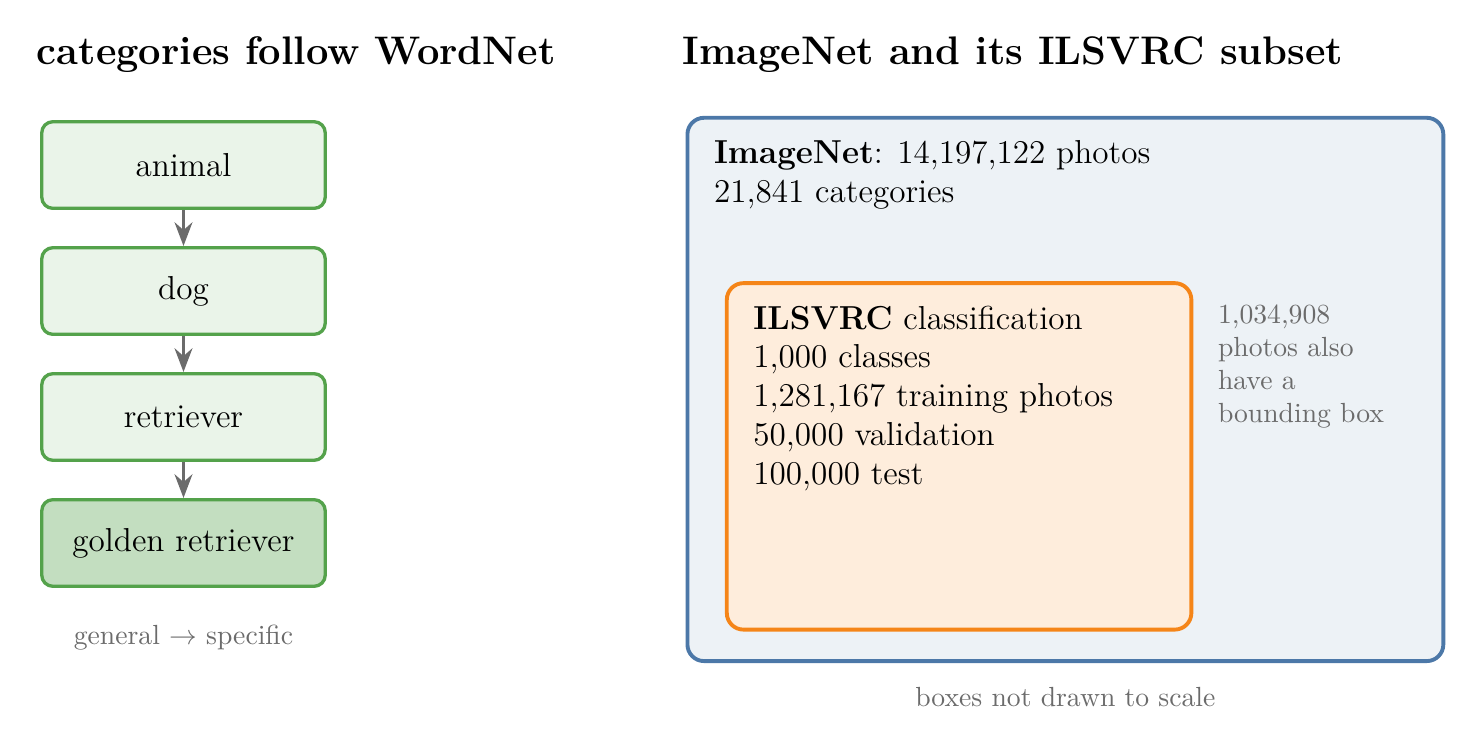
\begin{tikzpicture}[w/.style={box=cgreen, minimum width=3.6cm, font=\sffamily\large}]
  % WordNet hierarchy
  \node[title, anchor=west] at (-2.0,1.4) {categories follow WordNet};
  \node[w] (a) at (0,0) {animal};
  \node[w] (d) at (0,-1.6) {dog};
  \node[w] (r) at (0,-3.2) {retriever};
  \node[w, fill=cgreen!35] (g) at (0,-4.8) {golden retriever};
  \foreach \x/\y in {a/d,d/r,r/g} \draw[arrow] (\x) -- (\y);
  \node[note, font=\sffamily\normalsize] at (0,-6.0) {general $\rightarrow$ specific};
  % nested sets
  \begin{scope}[xshift=6.4cm]
  \node[title, anchor=west] at (-0.2,1.4) {ImageNet and its ILSVRC subset};
  \draw[cblue, fill=cblue!10, rounded corners=6pt, line width=1.4pt] (0,0.6) rectangle (9.6,-6.3);
  \node[anchor=north west, align=left, font=\sffamily\large] at (0.2,0.45)
    {\textbf{ImageNet}: 14,197,122 photos\\21,841 categories};
  \draw[corange, fill=corange!15, rounded corners=6pt, line width=1.4pt] (0.5,-1.5) rectangle (6.4,-5.9);
  \node[anchor=north west, align=left, font=\sffamily\large] at (0.7,-1.65)
    {\textbf{ILSVRC} classification\\1,000 classes\\1,281,167 training photos\\50,000 validation\\100,000 test};
  \node[anchor=north west, align=left, font=\sffamily\normalsize, text=cgrey] at (6.6,-1.65)
    {1,034,908\\photos also\\have a\\bounding box};
  \node[note, font=\sffamily\normalsize] at (4.8,-6.75) {boxes not drawn to scale};
  \end{scope}
\end{tikzpicture}
\end{document}
